%-----------------------------------------------------------------------
% RigidBodyMotion: discussion of the class that integrates the motion of rigid bodies.
%-----------------------------------------------------------------------

\section{Rigid Body Motion}\label{sec:rigidBodyMotion}

  This section discusses the motion of rigid bodies and the RigidBodyMotion class
that is used by Overture solvers to integrate the motion of rigid bodies.

The class {\tt RigidBodyMotion} can be used to track the motion
of a rigid body moving under the influence of forces and torques.

A {\tt RigidBodyMotion} object must be initialized with the basic
information about a body such as the mass, moments of inertia and
axes of inertia, in addition to the initial position and velocities.

A rigid body moves under the influence of a force, $\Fv(t)$ and torque $\Gv(t)$.
These forces and torques should be supplied at a sequence of times,
$(t_i,\Fv(t_i),\Gv(t_i))$. The rigid body object will integrate the equations
of motion and supply the currect position and orientation.

\newcommand{\mrb}{m_{b}}% position of the center of mass
\newcommand{\xvcm}{\xv_{\rm cm}}% position of the center of mass
\newcommand{\vvcm}{\vv_{\rm cm}}% velocity of the center of mass
\newcommand{\avcm}{\av_{\rm cm}}% acceleration of the center of mass

\newcommand{\dotxvcm}{\dot\xv_{\rm cm}}% position of the center of mass
\newcommand{\dotvvcm}{\dot\vv_{\rm cm}}% velocity of the center of mass

\subsection{Nomemclature}

Nomemclature:
\begin{alignat*}{3}
   \mrb             &\qquad&& \text{mass of the rigid body}\\
   \xvcm(t)        &\qquad&& \text{position of the center of mass} \\
   \vvcm(t)        &\qquad&& \text{velocity of the center of mass} \\
   \avcm(t)        &\qquad&& \text{acceleration of the center of mass} \\
  \Fv(t)            &\qquad&& \text{force on the body} \\
  \Gv(t)            &\qquad&& \text{torque on the body (about the center of mass)} \\
  \hv(t)            &\qquad&& \text{angular momentum} \\
  \ev_i(t)          &\qquad&& \text{principal axes of inertia, $i=1,2,3$.}\\
  \omegav(t)        &\qquad&& \text{angular velocity}\\
  E(t)\in \Real^{3\times3}        &\qquad&& \text{Matrix with columns $\ev_i$}\\
  R(t)\in \Real^{3\times3}        &\qquad&& \text{rotation matrix}\\
  A(t)\in \Real^{3\times3}        &\qquad&& \text{moment of inertial tensor}\\
  I_i            &\qquad&& \text{moments of inertia}
\end{alignat*}


% --------------------------------------------------------------------------------------------
\subsection{Motion of rigid bodies and the Newton-Euler equations}

Here we summarize the equations of motion for a rigid body which are known
as the Newton-Euler equations. See Section~\ref{sec:rigidBodyDynamics} for a derivation of the equations.


The equations of motion for a rigid body in the standard cartesian reference frame are
\begin{align*}
   \dotxvcm &= \vvcm , \\
   \mrb \dotvvcm &= \Fv ,\\
   \dot \hv &= \Gv , 
\end{align*}
where $\hv$ is the angular momentum (defined below). 
% where 
% \begin{align*}
% M  &  ~:~\mbox{mass of the body} \\
% \xv & ~:~\mbox{position of the centre of mass} \\
% \vv & ~:~\mbox{velocity of the centre of mass} \\
% \hv & ~:~\mbox{angular momentum} \\
% \Fv & ~:~\mbox{resultant force} \\
% \Gv & ~:~\mbox{resultant torque about the centre of mass} 
% \end{align*}
The force and torque are defined as 
\begin{align*}
   \Fv &= \int_{\partial\Omega} \fv_s\, ds + \fv_b, \quad \text{($\fv_s$ = surface forces, $\fv_b$= body force)},\\
   \Gv &= \int_{\partial\Omega} (\xv-\xvcm)\times\fv_s\, ds + \gv_b, \quad \text{(torque, $\gv_b$=body torque)}, 
%    \Gv &= \int_{\partial\Omega} (\rv -\xv_\cm) \times d\Fv, \qquad \mbox{torque on the body} ,
\end{align*}
where the integral is over the surface of the rigid body, $\partial\Omega$. The
contributions to the force and torque arise from forces on the surface of the body and external body forces. 
The angular momemtum $\hv$ is given by
\begin{align*}
   \hv & = A(t) \omegav 
\end{align*}
where $\omegav$ is the angular velocity,
and $A(t)$ is the moment of inertia tensor (wrt the center of mass) defined  by
\begin{align*}
   A(t) &= \int_{\Omega} \rho(\xv)\Big[ \yv^T\yv I - \yv\yv^T \Big] \, d\xv , \quad \yv = \xv-\xvcm, \quad \text{(inertia tensor)}. 
\end{align*}
Here $\rho(\xv)$ is the density (of mass) of the body.
$A(t)$ is a symmetric positive definite tensor with eigenvalues $I_i$ and eigenvectors $\ev_i$ (the principle axes of inertia), 
\begin{align*}
   A\ev_i &= I_i \ev_i, \quad \Lambda ={\rm diag}(I_1,I_2,I_3), \quad \ev_i\cdot\ev_j=\delta_{ij}, \\
   A &= E \Lambda E^T, \quad E =[\ev_1~ \ev_2~ \ev_3], \quad E^{-1}=E^T. 
\end{align*}
Note that $\Lambda$ does not depend on time.
The axes of inertia rotate with the body and thus
\begin{align*}
   \dot E &= \Omega E , \quad \dot\ev_i = \omegav\times\ev_i , \\
  \Omega & = \begin{bmatrix}
    0 & -\omega_3 & \omega_2 \\
    \omega_3 & 0 & -\omega_1 \\
    - \omega_2 & \omega_1  & 0 
\end{bmatrix}     , \quad \text{( i.e. $\Omega\av = \omegav\times\av$)}.
\end{align*}

From the definition of $\hv$ as $\hv = A(t) \omegav$, and the result $\dot A  = \Omega A - A \Omega$,
it follows that the evolution equation for the angular velocity
$\omegav$ is
\begin{align*}
   A \dot \omegav &= - \Omega A \omega + \Gv , \qquad \text{(angular velocity equation)}.
\end{align*}

% From $\hv & = A(t) \omegav$ and $A=E \Lambda E^T$ it follows that 
% \begin{align*}
%    \hv & = \sum I_i \omega_i \ev_i
% \end{align*}
% 
% 
% It is convenient to represent the angular momentum, $\hv$, in terms of the
% principle moments of inertia, $I_i$, the principle axes of inertia, $\ev_i=\ev_i(t)$, and the 
% angular velocities $\omegav_i$ about each axis $\ev_i$
% \begin{align*}
%    \hv & = \sum I_i \omega_i \ev_i \\
%    \ev_i\cdot\ev_j & = \delta_{ij}
% \end{align*}
% Since the principle axes of inertia remain an orthonormal basis it follows that
% \begin{align*}
%   \dot{\ev_i} &= \omegav\times\ev_i \qquad (\ev_i\cdot\ev_i=1, ~~\ev_i\cdot\dot{\ev}_i=0)
% \end{align*}
% % (where $\omegav$ is the angular velocity about $\ev_i$)
% and then the equation for the angular momentum becomes 
% \begin{align*}
%   I_i \dot{\omega}_i &+ \omegav\times\hv \cdot \ev_i = \Gv\cdot\ev_i \\
%   \dot{\ev_i} &= \omegav\times\ev_i \qquad (\ev_i\cdot\ev_i=1, ~~\ev_i\cdot\dot{\ev}_i=0)
% \end{align*}
% where the subscripts on $I$ and $\omega$ are to taken modulo 3 in the sense $I_{i+1}:=I_{(i{\rm mod} 3)+1}$.
% and where 
% \begin{align*}
% I_i & ~:~\mbox{principle moments of inertia} \\
% \ev_i & ~:~\mbox{principle axes of inertia} \\
% \omegav =(\omega_1,\omega_2,\omega_3) &  ~:~\mbox{angular velocities about $\ev_i$ } \\
% \end{align*}

In summary we solve the following set of ODEs
\begin{align}
   \dotxvcm &= \vvcm , \label{eq:rigidBodyX} \\
   \mrb \dotvvcm &= \Fv , \label{eq:rigidBodyV} \\
   A \dot \omegav &= - \Omega A \omega + \Gv , \qquad \text{(angular velocity equation)}, \label{eq:angularVelocity} \\
  \dot{\ev_i} &= \omegav\times\ev_i, \qquad (\ev_i\cdot\ev_i=1, ~~\ev_i\cdot\dot{\ev}_i=0)\label{eq:rigidBodyE}.
\end{align}
We integrate the motion of the principle axes, $\ev_i(t)$ over time in order to compute
the rotation matrix which is needed to find the positions, velocities and accelerations
of points attached to the body.
The rotation matrix that must be applied to rotate the body from it's position at $t=0$ to
any time $t$  is simply $E(t)E^T(0)$ where $E$ is the matrix
with columns being $\ev_i$,
\[
   R(t) = E(t) E^{-1}(0) = E(t)E^T(0).
\]
For a point $\rv(t)$ attached to the rigid body we have
\begin{align}
    \rv(t) &= \xvcm(t) + R(t) (\rv(0)-\xvcm(0)) .   \\
    \dot\rv(t) &= \vvcm(t) +\Omega R(t) (\rv(0)-\xvcm(0)) ,\\
               &= \vv(t) +\Omega (\rv(t)-\xvcm(t)) , \\
               &= \vv(t) +\omegav\times(\rv(t)-\xvcm(t)),\\
    \ddot\rv(t) &= \avcm(t) + \dot\omegav\times(\rv(t)-\xvcm(t)) + \omegav\times(\omegav\times(\rv(t)-\xvcm(t))), \\
                &= \avcm(t) + \dot\omegav\times(\rv(t)-\xvcm(t)) + (\omegav\cdot(\rv(t)-\xvcm(t)))\omegav - (\omegav\cdot\omegav)(\rv(t)-\xvcm(t))), 
\end{align}



% The rotation matrix that must be applied to rotate the body from it's position at $t=0$ to
% any time $t$  is simply $E(t)E^{-1}(0)$ where $E$ is the matrix
% with columns being $\ev_i$,
% \[
%    R(t) = E(t) E^{-1}(0) = \begin{bmatrix} \ev_0(t) & \ev_1(t) & \ev_2(t) \end{bmatrix}
%                           \begin{bmatrix} \ev_0^T(0) \\ \ev_1^T(0) \\ \ev_2^T(0) \end{bmatrix}
% \]
% Note that the inverse of $E$ is its transpose, $E^{-1}(t)=E^T(t)$. 
% 
% Thus the position, $\rv(t)$, of a point $\rv$ on the surface of the body will
% be given by the sum of the position of the centre of mass, $\xv(t)$ plus a rotation.
% \[
%     \rv(t) = \xv(t) + R(t) (\rv(0)-\xv(0))
% \]
% Whence the velocity and acceleration of the point are
% \begin{align*}
%   \dot{\rv}(t) &= \vv(t) + \dot{R} (\rv(0)-\xv(0)) \\
%                &= \vv(t) +\sum_i (\omegav\times\ev_i) (r_i(0)-x_i(0)) \\
%   \ddot{\rv}(t) &= \Fv/M + \ddot{R} (\rv(0)-\xv(0)) \\
%                 &= \Fv/M +\sum_i (\dot{\omegav}\times\ev_i+\omegav\times\dot{\ev_i}) (r_i(0)-x_i(0)) \\ 
%             &= \Fv/M +\sum_i (\dot{\omegav}\times\ev_i+\omegav\times(\omegav\times\ev_i)(r_i(0)-x_i(0)) \\ 
%      &= \Fv/M +\sum_i (\dot{\omegav}\times\ev_i+(\omegav\cdot\ev_i)\omegav+|\omegav|^2\ev_i)(r_i(0)-x_i(0)) 
% \end{align*}
% 



%- % ---------------------------------------------------------------
%- \subsubsection{Background}
%- 
%- Reference {\sl Fundamentals of Mechanics} by Synge and Griffith.
%- 
%- The angular momentum $\hv$ of a rigid body about it's centre of mass is 
%- \[
%-    \hv = \int_B (\rv -\xv_\cm) \times d\pv 
%- \]
%- where $d\pv$ is the momentum of a volume element and 
%- where the integral is over the volume occupied by the body.
%- 
%- Given a rigid body we can define the moment of inertial about a line $\lv$
%- to be 
%- \begin{align*}
%-       I &= \int_B m(\xv) r(\xv)^2 d\xv \\
%-       r &= | \hat{\lv} \times \xv |
%- \end{align*}
%- where $\hat{\lv}$ is a unit vector in the direction of $\lv$ and thus $r$ is the distance
%- from a point $\xv$ in the body to the line $\lv$.
%- 
%- We can define the principle moments of inertia and the principle axes of inertia as follows.
%- Define 
%- \begin{align*}
%-     A_{11} &=  \int_{B} m (x_2^2 + x_3^2) d\xv \\
%-     A_{22} &=  \int_{B} m (x_3^2 + x_1^2) d\xv \\
%-     A_{33} &=  \int_{B} m (x_1^2 + x_2^2) d\xv \\
%-     A_{13} &= -\int_{B} m  x_3 x_1        d\xv \\
%-     A_{12} &= -\int_{B} m  x_1 x_2        d\xv \\
%-     A_{23} &= -\int_{B} m  x_2 x_3        d\xv   
%- \end{align*}
%- The principle moments of inertia are the eigenvalues, $I_i$, of
%- \[
%-    A \ev = I \ev
%- \]
%- while the eigenvectors, $\ev_i$,  are the principle axes of inertia.
%- 
%- 
%- Let $\omegav=(\omega_1,\omega_2,\omega_3)$ be the angular velocities of the body about 
%- the principle axes of inertia. Let $\Omegav$ be the angular velocity of the principle
%- axes, $\ev_i$ (normally $\Omegav=\omegav$ but in symmetric problems we may not need to
%- rotate the some of the principle axes).
%- 
%- The equations of motion of the rigid body in the (rotating) reference frame attached to
%- the principle axes $\ev_i$
%- are
%- \begin{align*}
%-   M {d \vv \over dt} &= M\Big( {\partial \vv \over \partial t } + \Omegav\times\vv \Big) = \Fv \\
%-   {d  \hv\over dt} &= {\partial \hv \over \partial t }  + \Omegav\times\hv = \Gv
%- \end{align*}
%- where
%- \begin{align*}
%-    M &= \mbox{total mass of the body} \\
%-    \xv_\cm &= \mbox{center of mass} \\
%-    \vv &= \mbox{velocity of the center of mass} \\
%-    \hv &= \sum I_i \omega_i \ev_i  \qquad \mbox{angular momentum} \\
%-    \Fv &= \mbox{ external force on the body} \\
%-    \Gv &= \int (\rv -\xv_\cm) \times d\Fv \qquad \mbox{torque on the body} 
%- \end{align*}
%- 
%- Written out in components, the equations for the 6 degrees of freedom of a 
%- rigid body are
%- \begin{align*}
%-   M ( \dot{v}_1 - v_2 \Omega_3 + v_3 \Omega_2 ) &= F_1 \\
%-   M ( \dot{v}_2 - v_3 \Omega_1 + v_1 \Omega_3 ) &= F_2 \\
%-   M ( \dot{v}_3 - v_1 \Omega_2 + v_2 \Omega_1 ) &= F_3 \\
%-   I_1 \dot{\omega}_1 - I_2 \omega_2 \Omega_3 + I_3 \omega_3 \Omega_2 &= G_1 \\
%-   I_2 \dot{\omega}_2 - I_3 \omega_3 \Omega_1 + I_1 \omega_1 \Omega_3 &= G_2 \\
%-   I_3 \dot{\omega}_3 - I_1 \omega_1 \Omega_2 + I_2 \omega_2 \Omega_1 &= G_3 
%- \end{align*}
%- These equations need to be integrated to determine the coordinates of the centre of mass,
%- $\xv_\cm(t)$, and the angles of rotation $\thetav(t)$ ($\dot{\thetav}=\omegav$) about the principle axes.

% -----------------------------------------------------------------------------------
\subsection{Rigid body motion and the added mass matrices} \label{sec:rigidBodyAddedMass}


The force, $\Fv$, and torque, $\Gv$, can depend on the velocity, $\vvcm$, and angular velocity, $\omegav$, of the
rigid body (for example a drag force law may be of the form $\Fv = - C_d |\vvcm|^2$. In this case we may want to
explicitly expose this dependence when solving the equations of motion so that these terms can
be treated in an implicit fashion (for example). 

Therefore we write the equations in the form
\begin{align}
   \mrb \dotvvcm &=  -M_{11} \vvcm - M_{12} \omegav + \tilde{\Fv},  \\
   A \dot\omegav &=  -M_{12} \vvcm - M_{22} \omegav  -\dot A\omegav  + \tilde{\Gv}.
\end{align}
The matrices $M_{11}$, $M_{12}$, $M_{21}$, $M_{22}$ are called the added mass matrices. In general
they can depend on the solution, $M_{ij}=M_{ij}(\vvcm,\omegav,t)$. The added mass matrices can
be provided by the user when solving the rigid-body equations. 


% ================================================================================================
\subsection{Numerical integration of the Newton-Euler equations of motion}

The equations of motion are given by equations~\eqref{eq:rigidBodyX}-\eqref{eq:rigidBodyE}.
We can integrate these with any ODE method.
When the rigid-body is coupled to a fluid flow computation, the forces and torques will
only be available at certain discrete times. In addition the fluid equations are generally
solved with a predictor-corrector type scheme so it is convenient if the rigid body
equations can also be solved with a predictor-corrector scheme.

The time-stepping schemes available with the {\tt RigidBodyMotion} class are
\begin{description} 
  \item[LeapFrog-Trapezoidal] : a second-order accurate scheme, see Section~\ref{sec:leapFrogTrap}.
  \item[Implicit Runge Kutta] : DIRK schemes of order 1 to 4 have been implemented, 
            see Section~\ref{sec:DIRK}.
\end{description}


\subsubsection{A matlab code for integrating the Newton-Euler equations} \label{sec:matlabNewtonEuler}


The matlab code {\tt rigidBody.m} can be used to solve the Newton-Euler equations for 
rigid body motion. This code can be used to test various schemes. 
We solve the equations
\begin{align}
   \dotxvcm &= \vvcm , \\
   \mrb \dotvvcm &= \Fv ,\\
   \dot \hv &= \Gv , \\
   A \dot \omegav & = - \Omega A \omegav + \Gv , \\
   \dot E &= \Omega E ,\\
   \dot \qv &= [ 0,~ \omegav ] \qv . 
\end{align}
The last equation is that for the quaternion, which can be used in place of solving $\dot E = \Omega E$.
The quaternion is a vector in $\Real^4$ which is of unit length (for rotations). The number of
degrees of freedom in the unit-length quaternion thus equals the 3 degrees of freedom for rotations. 

The matlab code {\tt rigidBody.m} implements a variety of schemes,
\begin{description}
  \item [ode45] - use the matlab ode45 routine (a fourth-order RK scheme -- actually Dormand-Price now instead of Runge-Kutta Felhberg)
  \item[rk4] - solve use the standard fourth-order RK scheme.
  \item[leapFrogTrapPC] - the leapfrog predictor, trapezoidal rule correction (as found in the RigidBodyMotion class).
  \item[AMIleapFrogTrapPC] - a leapfrog predictor, trapezoidal rule correction scheme which treates the added mass
               terms implicitly.
  \item[DIRKj] - diagonally implicit Runge-Kutta schemes (orders j=1,2,3,4) that treat all terms implicitly (using Newton
         to solve the nonlinear equations at each stage). These schemes will work with the added mass terms, 
         even if the mass of the rigid body goes to zero.
\end{description}




% ------------------------------------------------------------------------------------------------------
\subsubsection{Leapfrog Trapezodial Predictor Corrector} \label{sec:leapFrogTrap}

The leapfrog-trapezodial scheme was the original scheme developed for the {\tt RigidBodyMotion} class.


The leapfrog-trapezodial scheme  consists of a predictor and a corrector step.
The {\bf predictor} step (implemented in the {\tt integrate} function of the RigidBodyMotion class)
is
\begin{align*}
    \vv^p &= \vv^{n-1} + 2\dt \fv^n \\
    \xv^p &= 2 \xv^n - \xv^{n-1} + \dt^2 \fv^n \\   
    \omegav^p &= \omegav^{n-1} + 2\dt \dot{\omegav}^n \\
    \ev^p &= \ev^{n-1} + 2\dt \dot{\ev}^n
\end{align*}
Here $\fv= \Fv/M$ is the force divided by the mass. The predictor is chosen to be a second-order
accurate leap-frog scheme.
The first two steps are treated in a special way as indicated below.
%  A forward-Euler predictor could also have been used and the
% overal scheme would r We choose a more accurate predictor 

The {\bf corrector} step (implemented in the {\tt correct} function) uses a trapezoidal
type approximation,
\begin{align}
    \vv^{n+1} &= \vv^{n} + \dt/2\Big( \fv^{n} + \fv^p \Big)  \label{eq:rbCorrectorV} \\
    \xv^{n+1} &= \xv^n   + \dt/2\Big( \vv^{n} + \vv^p \Big) \\
    \omegav^{n+1} &= \omegav^n + \dt/2 \Big( \dot{\omegav}^{n} + \dot{\omegav}^p \Big) \\
    \ev^{n+1} &= \ev^n + \dt/2 \Big( \dot{\ev}^{n} + \dot{\ev}^p \Big)
\end{align}


Question: Why have I chosen to integrate the both the equations for $\xv$ and $\vv$ ?


% In general the forces and torques acting on the rigid body may be functions of the current state, 

For the first step we use a locally second-order approximation to $\vv^1$ 
\begin{align*}
    \vv^{1} &= \vv^{0} + \dt \fv^0  \\
    \xv^{1} &= \xv^0   + \dt\Big( \vv^0 + \dt/2 \fv^0 \Big) \\
\end{align*}
Then on the second step we make a correction to $\vv^{1}$ making it locally $\dt^3$ accurate,
\begin{align*}
    \vv^{1} &= \vv^{0} + (\dt/2)\Big( \fv^n +\fv_{n+1} \Big) \\
\end{align*}
The equations for $\omegav^n$ and $\ev^n$ are treated in the same was as $\vv^n$.

*** check this is practice : what if we don't correct $\vv^1$ ??

%     v(R,next)=v0(R)+dt*vDot(R); // this is only first order but is fixed at second step.
%     x(R,next)=x(R,current)+dt*( v0(R) + .5*dt*vDot(R) );


If we suppose that $\fv=\fv(\vv,t)$ then the solution for $\vv^n$ is not directly coupled
to the other variables. 
% Note that when $\fv$ only depends on time that 
% $\vv^n$, $\wv^n$ and $\ev^n$ all evolve independently and thus
In this case the stability of the approach depends upon the stability of the leap-frog predictor and
Adams-Moulton corrector scheme (LFPC). 
For the ODE $y'=f(y)$ leap-frog predictor-corrector scheme reads
\begin{align*}
   y^p & = y^{n-1} + 2 f^n  \\
   y^{n+1} &= y^n + {\dt\over 2}( f^p + f^n)
\end{align*}
The stability region for this scheme is plotted in figure~\ref{fig:stabilityLFPC}.
For comparison we also show the stability region for the Adams predictor-corrector scheme (PC22),
\begin{align*}
   y^p & = y^{n-1} +  {3\over 2} \dt f^n - {1\over 2}\dt f^{n-1}  \\
   y^{n+1} &= y^n + {\dt\over 2}( f^p + f^n)
\end{align*}
Compared to the PC22 scheme, the stability region for the LFPC scheme includes a bit more
of the imaginary axis (i.e. it is good for oscillatory problems) but does not extend
as far into the left half plane. 
{
\newcommand{\figWidtha}{8cm}
\begin{figure}[hbt]
  \begin{center}
   % \epsfig{file=\obDir/doc/leapFrogCorrector.ps,width=.49\linewidth}
   % \epsfig{file=\obDir/doc/pece22withAxes.ps,width=.49\linewidth}
   \includegraphics[width=\figWidtha]{figures/leapFrogCorrector}
   \includegraphics[width=\figWidtha]{figures/pece22withAxes}
  \end{center}
\caption{Stability region for the leap-frog predictor corrector (LFPC) scheme (left) and a second-order
    Adams predictor corrector (PC22) scheme (right).}\label{fig:stabilityLFPC}
\end{figure}
}

% ----------------------------------------------------------------------------------------------
\subsubsection{Diagonally implicit Runge-Kutta (DIRK) schemes}  \label{sec:DIRK}

In order to solve the Newton-Euler equations with added mass terms, even when the mass of the
rigid body goes to zero, we need to use implicit schemes. Implicit Runge-Kutta schemes are a possible solution.


The diagonally implicit Runge-Kutta schemes (with $s$ stages) for solving $\dot \yv=\fv(\yv,t)$ are of the form
\begin{align}
   \kv_i &= \fv(\yv^n + \dt \sum_{j=1}^i a_{ij} \kv_j, t+c_i\dt),   \label{eq:kRK} \\
   \yv^{n+1} &= \yv^n + \dt \sum_{j=1}^s b_i \kv_i .
\end{align}
The schemes are implicit if $a_{ii}\ne 0$. 

For the case of light bodies with added mass we wish to solve the ODE's
\begin{align}
   \mrb \dotvvcm &= -A_{11}\vvcm - A_{12}\omegav + \Fv ,\\
   A(E) \dot \omegav & = - \Omega(\omegav) A \omegav -A_{21}\vvcm - A_{22}\omegav + \Gv , \\
   \dot E &= \Omega E ,
\end{align}
which can be written in the form ($\yv=[ \vvcm, ~ \omegav,~ E]^T$), 
\begin{align}
&   M(\yv) \dot \yv  = \fv(\yv,t) , \\ 
&   M = \begin{bmatrix}
             \mrb I_{3\times3} & \zerov & \zerov\\
             \zerov & A(E)  & \zerov \\
             \zerov & \zerov & I_{9\times9}
        \end{bmatrix}.
\end{align}
where the {\em mass} matrix $M$ could be singular (if $\mrb$ goes to zero or the inertia matrix A(E) becomes singular). 
% 
In this case, instead of solving~\eqref{eq:kRK}, we instead solve,
\begin{align}
   M(\yv^n + \dt \sum_{j=1}^i a_{ij} \kv_j) ~\kv_i &= \fv(\yv^n + \dt \sum_{j=1}^i a_{ij} \kv_j, t+c_i\dt).
\end{align}
These implicit equations can have a solution for $\kv_i$ even if $M$ is singular.
We thus require the solution to the nonlinear equations
\begin{align}
 \Fc(\zv) &= \begin{bmatrix} \Fc^{\vv}(\zv) \\  \Fc^{\omegav}(\zv)\\ \Fc^{E}(\zv) \end{bmatrix} = 0, \label{eq:NEnonlinear}
\end{align}
where
\begin{align}
 \Fc(\zv) &\equiv  M(\zv) ( \zv - \bar \zv)  - a_{ii}\dt \fv(\zv , t+c_i\dt), \\
 & \bar \zv \equiv \yv^n + \dt \sum_{j=1}^{i-1} a_{ij} \kv_j .
\end{align}
The quantity $\kv_i$ is then given by $\kv_i = ( \zv - \bar \zv)/( a_{ii}\dt)$. 
% 
To be specific, if $\zv=[\vv,~\omegav,~E]$, the equations we solve are 
\begin{align}
  \Fc^{\vv}(\zv) &= \mrb (\vv -\bar\vv) - a_{ii}\dt\Big( -A_{11}\vv - A_{12}\omegav + \Fv(t+c_i\dt)\Big) ,\\
  \Fc^{\omegav}(\zv) &= A(E) (\omegav-\bar\omegav) 
               - a_{ii}\dt\Big( -\Omega(\omegav) A(E) \omegav - A_{21}\vv - A_{22}\omegav + \Gv(t+c_i\dt)\Big) , \\
  \Fc^{E}(\zv) &=  (E-\bar E) - a_{ii}\dt \Big(  \Omega(\omegav) E\Big) ,
\end{align}
% 
We solve~\eqref{eq:NEnonlinear} by Newton's method. If $\zv^k$ is the current guess then the
new estimate $\zv^{k+1}$ satisfies
solve
\begin{align}
  \frac{\partial \Fc}{\partial \zv}(\zv^k) (\zv^{k+1}-\zv^k) &= - F(\zv^k).
\end{align}
To evaluate the Jacobian matrix we require $\partial (A(E) \omegav)/\partial E$. 
However, since $E$ has columns $\ev_j$, $j=1,2,3$, 
\begin{align}
   \Gc &\equiv  A(E) \omegav = E \Lambda E^T \omegav = \sum_{j=1}^3 \lambda_j (\ev_j^T\omegav) \ev_j . 
\end{align}
whence, 
\begin{align}
   \frac{\partial \Gc}{\partial \ev_k}  &=  \lambda_k\Big(  (\ev_k^T\omegav) I_{3\times3} + \ev_k\omega^T \Big). 
\end{align}
Also note that (since $\Omega A \omega = \omegav\times A \omegav = - (A\omegav)\times\omegav$), 
\begin{align}
   \frac{\partial (\Omega A \omega)}{\partial \omegav}  &=  \Omega A - [ A\omegav\times].
\end{align}


\subsubsection{DIRK schemes of orders 1 to 4}

The coefficients $a_{ij}$, $b_i$ and $c_i=\sum_j a_{ij}$ can be written in a Butcher tableau, 
\renewcommand{\arraystretch}{1.5}
\begin{align}
 \begin{array}{c|c}
  \cv & [a_{ij}] \\
  \hline
     & \bv^T
 \end{array}
\end{align}

A first order DIRK scheme (denoted by DIRK1) is the backward Euler scheme, with tableau
\begin{align}
 \begin{array}{c|c}
  1 & 1 \\
  \hline
     & 1
 \end{array}
\end{align}
A one-stage ($s=1$) second-order DIRK scheme (denoted by DIRK2) is the implicit mid-point rule with coefficients,
\begin{align}
 \begin{array}{c|c}
  \half & \half \\
  \hline
     & 1
 \end{array}
\end{align}
A two-stage third-order (A-stable) scheme (denoted by DIRK3) due to Crouzeiux is
\begin{align}
 \begin{array}{c|cc}
  \half+\frac{1}{2\sqrt{3}} & \half+\frac{1}{2\sqrt{3}} &       0                     \\
  \half-\frac{1}{2\sqrt{3}} & -\frac{1}{\sqrt{3}}       & \half+\frac{1}{2\sqrt{3}}   \\
  \hline
     & \half & \frac{1}{3} 
 \end{array}
\end{align}
This above scheme is also S-stable (see Alexander, SIAM J. Num. Anal. 1977) .
A four-stage fourth-order (A0-stable ?) scheme (denoted by DIRK4) due to Jackson and Norsett (1990) is
\begin{align}
 \begin{array}{c|cccc}
         1          &          1                &                      &                &         \\
   \frac{3}{5}      &          0                & \frac{3}{5}          &                &          \\
         0          &   \frac{171}{44}          & -\frac{215}{44}      &     1          &       \\
   \frac{2}{5}      &  -\frac{43}{20}           & \frac{39}{20}        &     0          &   \frac{3}{5}   \\
  \hline
                    & \frac{11}{72}             & \frac{25}{72}        & \frac{11}{72}  & \frac{25}{72}            
 \end{array}
\end{align}
This scheme has the property that the first two stages can be computed in parallel, and then the
last two stages can also be computed in parallel (due to $a_{21}=0$ and $a{4,3}=0$).


{\bf To-do:} Look for L-stable fourth-order schemes by Iserles and Norsett (1990)




% -----------------------------------------------------------------------------------------------------------
\subsection{Forcing relaxation for light bodies}\label{sec:lightBodyForcingRelaxation}

The simulation of the coupled motion of fluids and ``light'' rigid bodies can be
difficult since the standard time stepping algorithms can be unstable. The reason for this
instablility is discussed further in section~\ref{sec:lightBodies}.

One way to stabilize the time-stepping algorithm is to perform extra corrector iterations and
relax the forcing and torques provided to the rigid body corrector step. 

Thus the single corrector step~\eqref{eq:rbCorrectorV} (for simplicity we just consider the equation 
of the velocity here)
\begin{align}
    \vv^{n+1} &= \vv^{n} + \dt/2\Big( \fv^{n} + \fv^p \Big)  
\end{align}
is replaced by an iteration 
\begin{align}
    \vv^{n+1,k} &= \vv^{n} + \dt/2\Big( \fv^{n} + \fv^{n+1,k} \Big)  . 
\end{align}
Let $\tilde{\fv}^{k}$ denote the values for the forcing at correction step $k$, $k=1,2,\ldots$ (provided from a fluid solver
by integrating the tractions on the boundary for e.g.). Thus $\tilde{\fv}^{1}=\fv^p$. 
The actual forcing used to evolve the rigid body is 
\begin{align}
    \fv^{n+1,k} &= (1-\alpha)\fv^{n+1,k-1} + \alpha \tilde{\fv}^{k}, 
\end{align}
where $\fv^{n+1,0}$ is defined by extrapolation in time from previous values. For a constant time step this is 
\[
 \fv^{n+1,0}=2\fv^{n}-\fv^{n-1}.
\]
The relaxation parameter $\alpha$ should satisfy $\alpha\in (0,1]$.  Smaller values of $\alpha$ are required for 
lighter bodies. For example, the one-dimensional analysis of section~\ref{sec:lightBodies} suggests that
\begin{align}
    \alpha \le {2 \over 1 + M_s/(\rho_f V_f) } 
\end{align}
where $M_s$ is the mass of the body, $\rho_f$ is the density of the fluid and $V_f$ is some fluid volume corresponding to
the amount of fluid moved by the body. In practice one can choose a value for $\alpha$ and check whether the 
correction iterations converge. Choosing a very small value of $\alpha$ should always work but will require
more iterations to converge. Thus $\alpha$ should be chosen not too small. 

The correction steps are assumed to converge when the absolute or relative change in the force falls below given values, 
\begin{align}
    \Delta f^k  &< \tau_a, \text{~~or~~} { \Delta f^k \over \vert \tilde{\fv}^{k} \vert +\eps_f} < \tau_r , \quad\text{(convergence critera)}, \\
    \Delta f^k  &=  \vert \fv^{n+1,k} - \tilde{\fv}^{k} \vert.
\end{align}
The values for $\alpha$, $\tau_a$ and $\tau_r$ can be specified when defining the properties of the rigid body.


The torques, $\dot{\omegav}^p$, must also be under-relaxed for light bodies. The stability of the rotational motion depend on the
moment of inertia's (instead of the mass of the body). The torques have their own relaxation parameter and convergence
tolerances.


% --------------------------------------------------------------------------------------------------
\subsection{Exact and manufactured solutions to the Newton-Euler equations}


For verification of the numerical approximations we consider some exact or manufactured solutions.

\subsubsection{Trigonometric twilight zone solution (TZTrig)}

  The TZTrig exact solution for $\xvcm$, $\vvcm$ and $\omegav$ is 
\begin{align}
   v_i^{e}(t) & = a_i^v \cos( b_i^v ( t - c_i^v ) ) , \\
  \omega_i^{e}(t) & = a_i^\omega \cos( b_i^\omega( t - c_i^\omega) ),  \\
   x_i^{e}(t) & = \frac{a_i^v}{b_i^v} \sin( b_i^v ( t - c_i^v ) ) . 
\end{align}
The forcing and torque are then given by 
\begin{align}
   \Fv(t) &= \mrb \dot\vv^{e}, \\
   \Gv(t) &= A \dot\omegav^{e} + \Omega(\omegav^e) A \omegav^{e}, 
\end{align}
where the inertia matrix $A$ is evaluated from the current {\em numerical} solution. We do this to avoid
adding forcing functions to the $E$ equation. 

\subsubsection{Free rotation exact solutions (FR1, FR2, FR3)} 

In the frame of reference rotating with the body, the equations for $\hat\omega_i = \ev_i\cdot\omegav$ are 
\begin{align*}
  I_k \dot{\hat\omega}_k  &= (I_{k+1}-I_{k+2}) \hat\omega_{k+1}\hat\omega_{k+2}  + \ev_k^T\Gv,
\end{align*}
where the subscripts are cyclic, $I_{k+3} = I_{k}$,  (e.g. $I_{4}=I_{1}$).
With zero torque $\Gv=0$, and choosing $I_1=I_2$,  then $\dot{\hat\omega}_3=0$ and 
\begin{align*}
  \ddot{\hat\omega}_j  &= -\alpha^2 {\hat\omega}_j , ~~j=1,2, \\
  \alpha &= \Big\vert \frac{I_3-I_1}{I_1} {\hat\omega}_3(0) \Big\vert,
\end{align*}
with solution
\begin{align*}
  {\hat\omega}_1 &= A \cos(\alpha t) - C\sigma \sin(\alpha t), \\
  {\hat\omega}_2 &= C \cos(\alpha t) + A\sigma \sin(\alpha t), \\
  \sigma &\equiv \sgn(\frac{I_3-I_1}{I_1} {\hat\omega}_3(0)).
\end{align*}
This exact solution will be denoted as FR3 since ${\hat\omega}_3$ is constant. We can also define
exact solutions FR1 and FR2 by a cyclic permutation of the subscripts $j$ of ${\hat\omega}_j$ . 

It seems difficult to compute the exact solutions for $\omegav$ (or  $E$)
with this given solution for $\hat{\omegav}$ and thus we instead compute the error in $\hat{\omegav}$
from the computed values for $\ev_i\cdot\omegav$. 


\subsubsection{Quadratic drag law.}

An exact solution can be derived for a body falling through a fluid under the force of gravity where
the effect of the fluid is modeled with a simple drag law.
If the force on the body is due to gravity and a quadratic drag
\begin{align*}
  \Fv &= \mrb \gv -  C_D |\vvcm|^2\,\hat{\vv}_{\rm cm} , \quad \hat{\vv}_{\rm cm} =\frac{\vvcm}{|\vvcm|},\\
  \Gv &= \zerov,
\end{align*}
then the exact solution is
\begin{align*}
  \vvcm &= \alpha\tanh(\beta t)~\hat\gv  , \\
  \xvcm &= \frac{\alpha}{\beta} \log(\cosh(\beta t)) ~\hat\gv, \\
  \alpha &= \sqrt{\frac{\mrb |\gv|}{C_D}}, \quad \beta =\sqrt{\frac{C_D |\gv|}{\mrb}}, \quad \hat\gv=\frac{\gv}{|\gv|}.
\end{align*}
Note that $\alpha\beta=|\gv|$. We see that the velocity approaches the steady state value of $\alpha\hat\gv$.

An added mass matrix can be used in this example. In this case we
set
\begin{align*}
  \Fv &= m \gv - A_{11}\vvcm  ,\\
  A_{11} & = C_D\, \hat{\vv}_{\rm cm}\vvcm^T .
\end{align*}
We should be able to solve this problem with an implicit scheme  even if $\mrb\rightarrow 0$.

% --------------------------------------------------------------------
\subsection{Numerical Results}



\subsubsection{Solution for a sinusoidal forcing}


In this example we choose the forcing and torques to be 
\[
  \Fv = \begin{bmatrix}  
     c_1 \sin( f_1\pi t) \\
     c_2 \sin( f_2\pi t) \\
     c_3 \sin( f_3\pi t)    
    \end{bmatrix}  
   ,\qquad
  \Gv = \begin{bmatrix}
    c_4 \cos( f_1\pi t) \\ 
    c_4 \cos( f_2\pi t) \\ 
    c_6 \cos( f_3\pi t)    
  \end{bmatrix} 
\]


Figure~\ref{fig:generalSolution} shows the solution for $c_1=2$, $c_2=1.5$, $c_3=-1$,
$f_1=1$, $f_2=2$, $f_3=.5$ with $\xv(t_0)=0$, $\vv(t_0)=0$. 
$\ev(t_0)=I$, $I_1=1$, $I_2=.5$ and $I_3=2$. 


%- \begin{figure}[hbt]
%-   \begin{center}
%-    \epsfig{file=\obDir/doc/rigidBodyGeneralx.eps,width=.49\linewidth}
%-    \epsfig{file=\obDir/doc/rigidBodyGeneralw.eps,width=.49\linewidth}
%-    \epsfig{file=\obDir/doc/rigidBodyGenerale.eps,width=.49\linewidth}
%-   \end{center}
%- \caption{Solution to the Newton-Euler equations for a sinusoidal forcing.}\label{fig:generalSolution}
%- \end{figure}

The exact solution for $\xv$ and $\vv$ are easily determined ,
\begin{align*}
    x_n(t) &= -c_n \sin( f_n\pi t)/((f_n\pi)^2 M)
                    + (v_n(t_0) + c_n \cos( f_n\pi t_0)/(f_n\pi M) ) t + x_n(t_0) \\
    v_n(t) &= c_n (1-\cos(f_1\pi t))/(f_1\pi M)  + v_n(t_0)
\end{align*}

Although the evolution of the angular momentum $\hv$ can be determined analytically,
the evolution equations for $\omega$ and $\ev$ are nonlinear and I do not know how
to obtain the exact analytic solution. Instead we solve the equations independently 
using a matlab program with a fourth-order accurate Runge-Kutta scheme and a small
error tolerance. The errors in the predictor-correct scheme compared to
the very accurate results from the Runge-Kutta scheme are plotted in figure~\ref{fig:generalSolutionErr}.
(The maximum errors in the RK solution for $x_1$, $x_2$, $x_3$ are 
$1.37e-12$, $1.28e-11$, and $9.21e-14$). 

%- \begin{figure}[hbt]
%-   \begin{center}
%-    \epsfig{file=\obDir/doc/rigidBodyGeneralx-err.eps,width=.49\linewidth}
%-    \epsfig{file=\obDir/doc/rigidBodyGeneralw-err.eps,width=.49\linewidth}
%-    \epsfig{file=\obDir/doc/rigidBodyGenerale-err.eps,width=.49\linewidth}
%-   \end{center}
%- \caption{Errors in the predictor-corrector solution
%-     to the Newton-Euler equations for a sinusoidal forcing with $\Delta t=.005$.}\label{fig:generalSolutionErr}
%- \end{figure}


The maximum errors for $t\in[0,5]$ for two different values of $\delta t$ are given in table~\ref{tab:generalErr}.

\begin{table}[hbt]
\begin{center}
\begin{tabular}{|l|c|c|c|c|c|} \hline\hline 
   \multicolumn{4}{|c|}{Newton-Euler Equations} \\ \hline 
        & \multicolumn{2}{|c|}{Maximum errors}  &         \\ \hline 
        & $\Delta t=.005$ & $\Delta t=.0025$ & ratio   \\ \hline 
 $x_1$  & $1.31e-04$  & $3.27e-05$  & $4.00$ \\  
 $x_2$  & $1.96e-04$  & $4.90e-05$  & $4.00$ \\  
 $x_3$  & $3.68e-05$  & $9.22e-06$  & $4.00$ \\  
 $v_1$  & $3.93e-05$  & $9.82e-06$  & $4.00$ \\  
 $v_2$  & $5.89e-05$  & $1.47e-05$  & $4.00$ \\  
 $v_3$  & $9.82e-06$  & $2.45e-06$  & $4.00$ \\  
 $\omega_1$  & $3.76e-05$  & $9.49e-06$  & $3.96$ \\  
 $\omega_2$  & $2.99e-05$  & $7.44e-06$  & $4.02$ \\  
 $\omega_3$  & $1.43e-05$  & $3.49e-06$  & $4.09$ \\  
 $e_{11}$  & $3.31e-05$  & $8.17e-06$  & $4.05$ \\  
 $e_{12}$  & $3.77e-05$  & $9.45e-06$  & $3.99$ \\  
 $e_{13}$  & $2.50e-05$  & $6.31e-06$  & $3.97$ \\  
 $e_{21}$  & $1.87e-05$  & $4.67e-06$  & $4.01$ \\  
 $e_{22}$  & $2.17e-05$  & $5.54e-06$  & $3.92$ \\  
 $e_{23}$  & $2.34e-05$  & $5.92e-06$  & $3.96$ \\  
 $e_{31}$  & $2.39e-05$  & $5.93e-06$  & $4.04$ \\  
 $e_{32}$  & $2.22e-05$  & $5.40e-06$  & $4.11$ \\  
 $e_{33}$  & $3.82e-05$  & $9.50e-06$  & $4.02$ \\ 
\hline\hline 
\end{tabular}
\caption{Maximum errors for $t\in[0,5]$ in each solution component using the predictor-corrector method
    for the Newton-Euler equations for a sinusoidal forcing. The errors decrease by a factor
close to $4$ when $\Delta t$ is halved, indicating second-order accuracy.}\label{tab:generalErr}
\end{center}
\end{table}


% --------------------------------------------------------------------
\clearpage
\subsection{*NEW* Numerical Results}

\newcommand{\tableFont}{\small}
\input rigidBodyConv.tex



% ---------------------------------------------------------------------------------
\clearpage
\subsection{Derivation of the Rigid Body Equations of Motion} \label{sec:rigidBodyDynamics}



Consider a rigid body consisting of a set of $N$ particles connected by massless rods.
The particles have mass $m_i$, positions $\xv_i(t)$ and velocities $\vv_i(t)$. The equation of motion
for particle $i$ is given by Netwon's law
\begin{align*}
    m_i \ddot \xv_i = \fv_i + \sum_j \fv_{ij}
\end{align*}
where $\fv_i$ is the external force on the particle and $\fv_{ij}$ is the force exerted 
on particle $i$ from particle $j$ with $\fv_{ij}=-\fv_{ji}$.
By summing the equations of motions of the particles,
\begin{align*}
    \sum_{i=1}^N m_i \ddot \xv_i &= \sum_i \fv_i,  
\end{align*}
we obtain the equation of motion for the center of mass
\begin{align*}
    M \ddot \xv & = \fv, 
\end{align*}
where $M$ is the total mass and $\xv(t)$ is the position of the center of mass, 
\begin{align*}
    M &\equiv \sum_i m_i, \quad
    \xv = \frac{\sum_i m_i \xv_i}{\sum_i m_i} .
\end{align*}
Let $\yv_i=\xv_i-\xv$ denote the vector from particle $i$ to the center of mass.
Note that the length of $\yv_i$ is constant in time. This can be seen 
from
\begin{align*}
    M \yv_i &= \big(\sum_j m_j\big) \xv_i - \sum_j m_j \xv_j ~= \sum_j m_j( \xv_i-\xv_j) 
\end{align*}
Thus 
\begin{align*}
  M^2  \| \yv_i \|^2 &= M^2 \yv_i^T \yv_i = \Big\{ \sum_j m_j( \xv_i-\xv_j)^T \Big\} \Big\{ \sum_k m_k( \xv_i-\xv_k) \Big\}  \\
         &= M^2 \sum_j \sum_k m_j m_k ( \xv_i-\xv_j)^T( \xv_i-\xv_k)
\end{align*}
But $( \xv_i-\xv_j)^T( \xv_i-\xv_k) =\| \xv_i-\xv_j\| \|  \xv_i-\xv_k\| \cos(\theta) $ is constant in time since
the relative positions of the particles remains fixed in time.

Note that
% \begin{align*}
%     m_i \ddot \yv_i &=  m_i \ddot (\xv_i - \xv) = \fv_i + \sum_j \fv_{ij} - m_i \fv/M .
% \end{align*}
% and thus
% \begin{align*}
%    \sum_i  m_i \ddot \yv_i &=  \sum_i \fv_i + \sum_i \sum_j \fv_{ij} -  \sum_i m_i \fv/M ,
%                            &=0
% \end{align*}
% and therefore 
\begin{align*}
   \sum_i  m_i \yv_i &= \sum_i m_i (\xv_i -\xv) = M \xv - M \xv = 0,\\
   m_i \ddot \yv_i &=  m_i  (\ddot\xv_i - \ddot\xv) = \fv_i + \sum_j \fv_{ij} - m_i \fv/M .
\end{align*}

The equation for the angular momentum is found by summing $\yv_i\times m_i \ddot \yv_i$ ,
\begin{align}
    \sum_i m_i \yv_i\times \ddot \yv_i &= \sum_i \yv_i\times \fv_i  + \sum_i\sum_j \yv_i\times\fv_{ij} - \Big( \sum_i m_i \yv_i\times\Big) \fv/M,  \\
                    &= \sum_i \yv_i\times \fv_i \equiv \gv .  \label{eq:yTimesNewton}
\end{align}
Here $\gv$ is the torque about the center of mass.
The vectors $\yv_i(t)$ rotate about the origin as the rigid body rotates, 
\begin{align*}
    \yv_i(t) &= R(t) \yv_i(0),
\end{align*}
where $R(t)$ is a skew symmetric rotation matrix. The velocity $\dot\yv_i$ satisfies
\begin{align*}
  \dot\yv_i(t) &= \dot R(t) \yv_i(0) = \Omega R \yv_i(0) = \Omega \yv_i(t) = \omegav\times\yv_i(t),\\
   \dot R &= \Omega R,
 %   \ddot  \yv_i(t) &= \ddot R(t) \yv_i(0)
\end{align*}
where $\omegav$ is the {\em angular velocity} vector and $\Omega$ is the skew-symmetric matrix form of the cross product operator $\omegav\times$,
\begin{align*}
  \Omega & = \begin{bmatrix}
    0 & -\omega_3 & \omega_2 \\
    \omega_3 & 0 & -\omega_1 \\
    - \omega_2 & \omega_1  & 0 
\end{bmatrix} .
\end{align*}

Whence, from ~\eqref{eq:yTimesNewton} we obtain (note that $\dot\yv_i\times\dot\yv_i=0$), 
\begin{align*}
     \dot \hv &= \gv , \qquad   \hv = \sum_i m_i \yv_i\times \dot \yv_i
\end{align*}
where $\hv$ is defined to be the angular momentum. Now since $\av\times(\bv\times\cv) =(\av\cdot\cv)\bv - (\av\cdot\bv)\cv$
and $\dot\yv_i = \omegav\times\yv$, 
\begin{align*}
   \hv &= \sum_i m_i \yv_i\times \dot \yv_i = \sum_i m_i \yv_i\times( \omegav\times\yv), \\
       &= \sum_i m_i \big(  \yv_i^T\yv_i - \yv_i\yv_i^T\big) ~\omegav \\
       &= A(t)\, \omegav 
\end{align*}
where the symmetric positive definite matrix $A(t)$ is called the moment of inertial matrix,
\begin{align*}
  A(t) &= \sum_i m_i \big(  \yv_i^T\yv_i - \yv_i\yv_i^T \big), \\
      &= R(t) \Big[ \sum_i m_i \big(  \yv_i(0)^T\yv_i(0)  - \yv_i(0)\yv_i(0)^T\big) \Big] R^T(t),  \\
%       &= R(t) \Big\[ \sum_i m_i \big(  \yv_i(0)^T\yv_i(0)  - \yv_i(0)\yv_i(0)^T\big) \Big\] R^T(t),  \\
       &= R(t) A(0) R^T(t)
\end{align*}
If $A(0)$ has eigenvalues $I_i$ and eigenvectors $\ev_i(0)$ (of unit length), 
\begin{align*}
   A(0)\ev_i(0) = I_i \ev_i(0), ~~i=1,2,3, 
\end{align*}
then if $E(0)$ is the orthonormal matrix with columns $\ev_i(0)$ and $M_I$ is the diagonal matrix with entries $I_i$, 
\begin{align*}
   E_0 &= [\ev_1(0)~ \ev_2(0)~ \ev_3(0)], \qquad  M_I = {\rm diag}(I_1,I_2,I_3) , \\
   A(0)E(0) &= E(0) M_I, \\
   A(0) &= E(0) M_I E(0)^T , 
\end{align*}
then
\begin{align*}
  A(t) &= R(t)E(0) M_I (R(t)E(0))^T, \\
       &= E(t) M_I E(t)^T,   \\
  E(t) &=[\ev_1(t)~ \ev_2(t)~ \ev_3(t)] = R(t) [\ev_1(0)~ \ev_2(0)~ \ev_3(0)] = R(t) E_0, \\
    R(t)& = E(t)E^T(0).
\end{align*}

In summary, the equations of motion are
\begin{align*}
  M \ddot \xv &= \fv = \sum_i \fv_i \\
  \dot\hv &= \gv = \sum_i (\xv_i-\xv)\times\fv_i , \\
  \hv &= E(t) M_I E(t)^T\omegav~~ = \sum_{k=1}^3  I_k (\ev_k\cdot\omegav) \ev_k, \\
  \dot\ev_i &= \omegav\times\ev_i , \quad \dot E = \Omega E.
\end{align*}
and then the motion of a point $\pv$ on the body is given by
\begin{align*}
  \pv(t) &= \xv(t) + R(t) (\pv(0)-\xv(0)) , \\
 \dot\pv(t) &= \vv(t) + \Omega R(t) (\pv(0)-\xv(0)) \quad = \vv(t) + \Omega (\pv(t)-\xv(t)), \\
            &= \vv(t) + \omegav\times (\pv(t)-\xv(t)),\\
 R(t)& = E(t)E^T(0).
\end{align*}

We could just solve the ODEs for unknowns $\xv$, $\vv=\dot\xv$, $\hv$, and $\ev_i$, by
integrating the equations
\begin{align*}
  \dot \xv &= \vv , \\
  M \dot \vv &= \fv , \\
  \dot\hv &= \gv , \\
  \dot\ev_i &= \omegav\times\ev_i ,\quad   \omegav = E(t) M_I^{-1} E(t)^T\hv .
\end{align*}

Alternatively we can write an equation for $\omegav$.

Since
\begin{align*}
   \dot A  &= \dot E M_I E^T + E M_I \dot E^T \\
                  &= \Omega A - A \Omega
\end{align*}
then
\begin{align*}
  \dot A\omegav  &= \Omega A\omegav - A\Omega\omegav \\
         &= \Omega \hv - A (\omegav\times\omegav)\\
         &= \Omega A\omegav = \Omega \hv = \omegav\times\hv
\end{align*}
then equation for $\omegav$ is
\begin{align*}
 &  A \dot\omegav + \dot A \omega = \gv \\
 &  \dot\omegav = - A^{-1}\Omega A \omegav + A^{-1}\gv \\
 &  A = E M_I E^T, \quad A^{-1} = E M_I^{-1} E^T
 \end{align*}
Another form of the angular momentum equation is 
\begin{align*}
   \dot \hv = A \dot\omegav + \omega\times\hv = \gv 
\end{align*}


Another common approach is to write an equation for the angular 
velocity, $\hat\omegav$, in the rotating frame,  
\begin{align}
\hat\omegav = E^T\omegav, \qquad (\hat\omega_i = \ev_i\cdot\omegav),
\end{align}
Then $\hv=E M_I\hat\omegav$ and 
\begin{align*}
   \dot\hv &= E M_I\dot{\hat\omegav} + \dot E M_I\hat\omegav = \gv \\
  M_I \dot{\hat\omegav} &= E^T( - \Omega E M_I\hat\omegav ) + \Ev^T\gv \\
                     &= -E^T\Big[ \omegav\times\big( \sum_j I_j \hat\omega_j \ev_j\big) \Big] + E^T\gv
\end{align*}
Thus, using $\av\cdot(\bv\times\cv) = - \bv\cdot(\av\times\cv)$, it follows that $k^{\rm th}$ component
of this last equation is 
\begin{align*}
  I_k \dot{\hat\omega}_k  &= - \ev_k\cdot\Big[ \omegav\times\big( \sum_j I_j \hat\omega_j \ev_j\big) \Big] + \ev_k^T\gv \\
                      &= \omegav\cdot\sum_j I_j \hat\omega_j \ev_k\times\ev_j.
\end{align*}
This gives (since $\ev_1\times\ev_2=\ev_3$, $\ev_1\times\ev_3=-\ev_2$, etc.) 
\begin{align*}
  I_k \dot{\hat\omega}_k  &= (I_{k+1}-I_{k+2}) \hat\omega_{k+1}\hat\omega_{k+2}  + \ev_k^T\gv,
\end{align*}
where the subscripts are cyclic, $I_{k+3} = I_{k}$,  (e.g. $I_{4}=I_{1}$). 

